
\documentclass[10pt]{standalone}
\usepackage[utf8]{inputenc}
\usepackage{tikz}

% tikzlibrary.code.tex
%
% Copyright 2010-2011 by Laura Dietz
% Copyright 2012 by Jaakko Luttinen
%
% This file may be distributed and/or modified
%
% 1. under the LaTeX Project Public License and/or
% 2. under the GNU General Public License.
%
% See the files LICENSE_LPPL and LICENSE_GPL for more details.

% Load other libraries

%\newcommand{\vast}{\bBigg@{2.5}}
% newcommand{\Vast}{\bBigg@{14.5}}
% \usepackage{helvet}
% \renewcommand{\familydefault}{\sfdefault}

\usetikzlibrary{shapes}
\usetikzlibrary{fit}
\usetikzlibrary{chains}
\usetikzlibrary{arrows}

% Latent node
\tikzstyle{latent} = [circle,fill=white,draw=black,inner sep=1pt,
minimum size=20pt, font=\fontsize{10}{10}\selectfont, node distance=1]
% Observed node
\tikzstyle{obs} = [latent,fill=gray!25]
% Invisible node
\tikzstyle{invisible} = [latent,minimum size=0pt,color=white, opacity=0, node distance=0]
% Constant node
\tikzstyle{const} = [rectangle, inner sep=0pt, node distance=0.1]
%state
\tikzstyle{estado} = [latent,minimum size=8pt,node distance=0.4]
%action
\tikzstyle{accion} =[latent,circle,minimum size=5pt,fill=black,node distance=0.4]
\tikzstyle{fijo} =[latent,circle,minimum size=5pt,fill=black]


% Factor node
\tikzstyle{factor} = [rectangle, fill=black,minimum size=10pt, draw=black, inner
sep=0pt, node distance=1]
% Deterministic node
\tikzstyle{det} = [latent, rectangle]

% Plate node
\tikzstyle{plate} = [draw, rectangle, rounded corners, fit=#1]
% Invisible wrapper node
\tikzstyle{wrap} = [inner sep=0pt, fit=#1]
% Gate
\tikzstyle{gate} = [draw, rectangle, dashed, fit=#1]

% Caption node
\tikzstyle{caption} = [font=\footnotesize, node distance=0] %
\tikzstyle{plate caption} = [caption, node distance=0, inner sep=0pt,
below left=5pt and 0pt of #1.south east] %
\tikzstyle{factor caption} = [caption] %
\tikzstyle{every label} += [caption] %

\tikzset{>={triangle 45}}

%\pgfdeclarelayer{b}
%\pgfdeclarelayer{f}
%\pgfsetlayers{b,main,f}

% \factoredge [options] {inputs} {factors} {outputs}
\newcommand{\factoredge}[4][]{ %
  % Connect all nodes #2 to all nodes #4 via all factors #3.
  \foreach \f in {#3} { %
    \foreach \x in {#2} { %
      \path (\x) edge[-,#1] (\f) ; %
      %\draw[-,#1] (\x) edge[-] (\f) ; %
    } ;
    \foreach \y in {#4} { %
      \path (\f) edge[->,#1] (\y) ; %
      %\draw[->,#1] (\f) -- (\y) ; %
    } ;
  } ;
}

% \edge [options] {inputs} {outputs}
\newcommand{\edge}[3][]{ %
  % Connect all nodes #2 to all nodes #3.
  \foreach \x in {#2} { %
    \foreach \y in {#3} { %
      \path (\x) edge [->,#1] (\y) ;%
      %\draw[->,#1] (\x) -- (\y) ;%
    } ;
  } ;
}

% \factor [options] {name} {caption} {inputs} {outputs}
\newcommand{\factor}[5][]{ %
  % Draw the factor node. Use alias to allow empty names.
  \node[factor, label={[name=#2-caption]#3}, name=#2, #1,
  alias=#2-alias] {} ; %
  % Connect all inputs to outputs via this factor
  \factoredge {#4} {#2-alias} {#5} ; %
}

% \plate [options] {name} {fitlist} {caption}
\newcommand{\plate}[4][]{ %
  \node[wrap=#3] (#2-wrap) {}; %
  \node[plate caption=#2-wrap] (#2-caption) {#4}; %
  \node[plate=(#2-wrap)(#2-caption), #1] (#2) {}; %
}

% \gate [options] {name} {fitlist} {inputs}
\newcommand{\gate}[4][]{ %
  \node[gate=#3, name=#2, #1, alias=#2-alias] {}; %
  \foreach \x in {#4} { %
    \draw [-*,thick] (\x) -- (#2-alias); %
  } ;%
}

% \vgate {name} {fitlist-left} {caption-left} {fitlist-right}
% {caption-right} {inputs}
\newcommand{\vgate}[6]{ %
  % Wrap the left and right parts
  \node[wrap=#2] (#1-left) {}; %
  \node[wrap=#4] (#1-right) {}; %
  % Draw the gate
  \node[gate=(#1-left)(#1-right)] (#1) {}; %
  % Add captions
  \node[caption, below left=of #1.north ] (#1-left-caption)
  {#3}; %
  \node[caption, below right=of #1.north ] (#1-right-caption)
  {#5}; %
  % Draw middle separation
  \draw [-, dashed] (#1.north) -- (#1.south); %
  % Draw inputs
  \foreach \x in {#6} { %
    \draw [-*,thick] (\x) -- (#1); %
  } ;%
}

% \hgate {name} {fitlist-top} {caption-top} {fitlist-bottom}
% {caption-bottom} {inputs}
\newcommand{\hgate}[6]{ %
  % Wrap the left and right parts
  \node[wrap=#2] (#1-top) {}; %
  \node[wrap=#4] (#1-bottom) {}; %
  % Draw the gate
  \node[gate=(#1-top)(#1-bottom)] (#1) {}; %
  % Add captions
  \node[caption, above right=of #1.west ] (#1-top-caption)
  {#3}; %
  \node[caption, below right=of #1.west ] (#1-bottom-caption)
  {#5}; %
  % Draw middle separation
  \draw [-, dashed] (#1.west) -- (#1.east); %
  % Draw inputs
  \foreach \x in {#6} { %
    \draw [-*,thick] (\x) -- (#1); %
  } ;%
}


\usepackage[english]{babel}
\usepackage{tikz}
\usepackage{caption}
\usepackage{float} % para que los gr\'aficos se queden en su lugar con [H]
\usepackage{subcaption}

\usepackage[utf8]{inputenc}
\usepackage{url}
\usepackage{graphicx}
\usepackage{color}
\usepackage{amsmath} %para escribir funci\'on partida , matrices
\usepackage{amsthm} %para numerar definciones y teoremas
\usepackage[hidelinks]{hyperref} % para inlcuir links dentro del texto
%\usepackage{tabu} 
\usepackage{comment}
\usepackage{amsfonts} % \mathbb{N} -> conjunto de los n\'umeros naturales  
\usepackage{enumerate}
\usepackage{listings}
\usepackage[colorinlistoftodos, textsize=small]{todonotes} % Para poner notas en el medio del texto!! No olvidar hacer. 
\usepackage{framed} % Para encuadrar texto. \begin{framed}
\usepackage{csquotes} % Para citar texto \begin{displayquote}
\usepackage{varioref}
\usepackage{bm} % \bm{\alpha} bold greek symbol
\usepackage{pdfpages} % \includepdf
\usepackage[makeroom]{cancel} % \cancel{} \bcancel{} etc
\usepackage{wrapfig} % \begin{wrapfigure} Pone figura al lado del texto
\usepackage{mdframed}
\usepackage{algorithm}
\usepackage{quoting}
\usepackage{mathtools}	
\usepackage{paracol}

\newcommand{\vm}[1]{\mathbf{#1}}
\newcommand{\N}{\mathcal{N}}
\newcommand{\citel}[1]{\cite{#1}\label{#1}}
\newcommand\hfrac[2]{\genfrac{}{}{0pt}{}{#1}{#2}} %\frac{}{} sin la linea del medio

\newtheorem{midef}{Definition}
\newtheorem{miteo}{Theorem}
\newtheorem{mipropo}{Proposition}

\theoremstyle{definition}
\newtheorem{definition}{Definition}[section]
\newtheorem{theorem}{Theorem}[section]
\newtheorem{proposition}{Proposition}[section]


%http://latexcolor.com/
\definecolor{azul}{rgb}{0.36, 0.54, 0.66}
\definecolor{rojo}{rgb}{0.7, 0.2, 0.116}
\definecolor{rojopiso}{rgb}{0.8, 0.25, 0.17}
\definecolor{verdeingles}{rgb}{0.12, 0.5, 0.17}
\definecolor{ubuntu}{rgb}{0.44, 0.16, 0.39}
\definecolor{debian}{rgb}{0.84, 0.04, 0.33}
\definecolor{dkgreen}{rgb}{0,0.6,0}
\definecolor{gray}{rgb}{0.5,0.5,0.5}
\definecolor{mauve}{rgb}{0.58,0,0.82}

\lstset{
  language=Python,
  aboveskip=3mm,
  belowskip=3mm,
  showstringspaces=true,
  columns=flexible,
  basicstyle={\small\ttfamily},
  numbers=none,
  numberstyle=\tiny\color{gray},
  keywordstyle=\color{blue},
  commentstyle=\color{dkgreen},
  stringstyle=\color{mauve},
  breaklines=true,
  breakatwhitespace=true,
  tabsize=4
}

\makeatletter
\newcommand{\vast}{\bBigg@{2.5}}
\newcommand{\Vast}{\bBigg@{14.5}}
\makeatother


\tikzstyle{arrow}= [thick, ->, >=stealth]
\usetikzlibrary{shapes.geometric, arrows}
\tikzstyle{operator}=[circle, radius= 0.2 cm, text centered, draw=black]


\usepackage{helvet}
\renewcommand{\familydefault}{\sfdefault}
\begin{document}
 
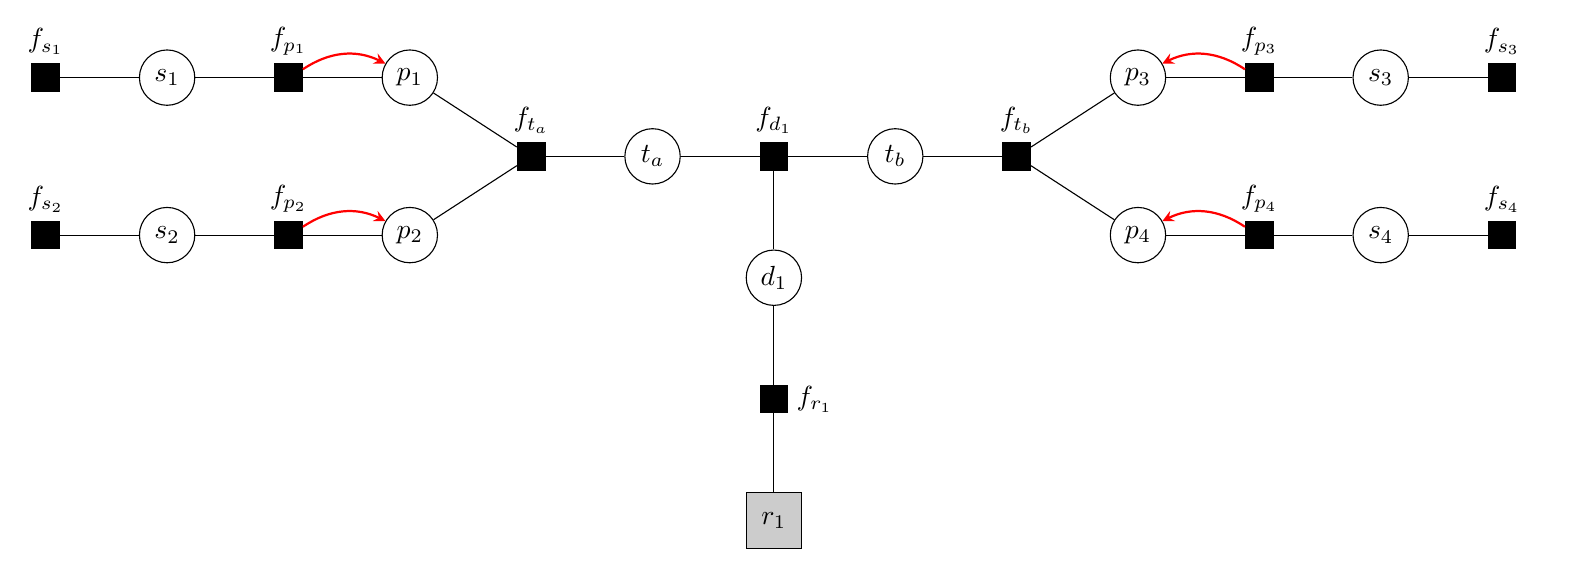
\begin{tikzpicture}

  [
    ->,
    >=stealth',
    auto,node distance=3cm,
    thick,
    main node/.style={circle, draw, font=\sffamily\Large\bfseries}
    ]
        
      
\node[det, fill=black!20] (r) {$r_1$};
      
        \node[factor, above=of r] (fr) {} ;
        \node[const, right=of fr] (nfr) {$f_{r_1}$}; %
	
	\node[latent, above=of fr] (d) {$d_1$} ; %
        \node[factor, above=of d] (fd) {} ;
        \node[const, above=of fd] (nfd) {$f_{d_1}$}; %
	
        
        \node[latent, left=of fd] (ta) {$t_a$} ; %
        \node[factor, left=of ta] (fta) {} ;
        \node[const, above=of fta] (nfta) {$f_{t_a}$}; %
        
        
        
        \node[latent, left=of fta,yshift=1cm] (p1) {$p_1$} ; %
        \node[factor, left=of p1] (fp1) {} ;
        \node[const, above=of fp1] (nfp1) {$f_{p_1}$}; %
        
        \node[latent, left=of fp1] (s1) {$s_1$} ; %
        \node[factor, left=of s1] (fs1) {} ;
	\node[const, above=of fs1] (nfs1) {$f_{s_1}$}; %
     
        \node[latent, left=of fta,yshift=-1cm] (p2) {$p_2$} ; %
        \node[factor, left=of p2] (fp2) {} ;
        \node[const, above=of fp2] (nfp2) {$f_{p_2}$}; %
        
        \node[latent, left=of fp2] (s2) {$s_2$} ; %
        \node[factor, left=of s2] (fs2) {} ;
	\node[const, above=of fs2] (nfs2) {$f_{s_2}$}; %
        
            
        \node[latent, right=of fd] (tb) {$t_b$} ; %
        \node[factor, right=of tb] (ftb) {} ;
        \node[const, above=of ftb] (nftb) {$f_{t_b}$}; %
        
        \node[latent, right=of ftb,yshift=1cm] (p3) {$p_3$} ; %
        \node[factor, right=of p3] (fp3) {} ;
        \node[const, above=of fp3] (nfp3) {$f_{p_3}$}; %
        
        \node[latent, right=of fp3] (s3) {$s_3$} ; %
        \node[factor, right=of s3] (fs3) {} ;
	\node[const, above=of fs3] (nfs3) {$f_{s_3}$}; %
     
        \node[latent, right=of ftb,yshift=-1cm] (p4) {$p_4$} ; %
        \node[factor, right=of p4] (fp4) {} ;
        \node[const, above=of fp4] (nfp4) {$f_{p_4}$}; %
        
        \node[latent, right=of fp4] (s4) {$s_4$} ; %
        \node[factor, right=of s4] (fs4) {} ;
	\node[const, above=of fs4] (nfs4) {$f_{s_4}$}; %
     
        \node[invisible, xshift=10cm] (i) {};
     
        \edge[-] {r} {fr};
        \edge[-] {fr} {d};
	\edge[-] {d} {fd};
	
        \edge[-] {fd} {ta};
        \edge[-] {ta} {fta};
        \edge[-] {fta} {p1};
        \edge[-] {p1} {fp1};
        \edge[-] {fp1} {s1};
        \edge[-] {s1} {fs1};
        \edge[-] {fta} {p2};
        \edge[-] {p2} {fp2};
        \edge[-] {fp2} {s2};
        \edge[-] {s2} {fs2};
        	
	\edge[-] {fd} {tb};
        \edge[-] {tb} {ftb};
        \edge[-] {ftb} {p3};
        \edge[-] {p3} {fp3};
        \edge[-] {fp3} {s3};
        \edge[-] {s3} {fs3};
        \edge[-] {ftb} {p4};
        \edge[-] {p4} {fp4};
        \edge[-] {fp4} {s4};
        \edge[-] {s4} {fs4};
        
        \path (fp1) edge[bend left, arrow,  color=red] node [right] {} (p1);
        \path (fp2) edge[bend left, arrow,  color=red] node [right] {} (p2);	      
        \path (fp3) edge[bend right, arrow,  color=red] node [left] {} (p3);
        \path (fp4) edge[bend right, arrow,  color=red] node [left] {} (p4);
\end{tikzpicture}

        
\end{document}

